\documentclass[border=4pt]{standalone}
\usepackage{tikz}
\usetikzlibrary{arrows.meta,calc,shapes.multipart}
\begin{document}
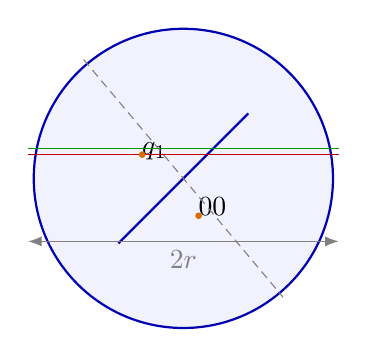
\begin{tikzpicture}[>=Latex]
  \node[shape=circle solidus,draw=blue!70!black,thick,
    fill=blue!5,inner xsep=7pt,inner ysep=5pt,outer sep=2pt,
    minimum size=38mm] (state)
    {$q_1$\nodepart{lower}$00$};

  \draw[red!75!black] (state.base west) -- (state.base east);
  \draw[green!60!black] (state.mid west) -- (state.mid east);
  \draw[gray,densely dashed] (state.130) -- (state.-50);
  \fill[orange!85!black] (state.text) circle (1.2pt)
    (state.lower) circle (1.2pt);
  \draw[<->,gray] ($(state.west)+(0,-8mm)$) --
    node[below] {$2r$} ($(state.east)+(0,-8mm)$);
\end{tikzpicture}
\end{document}
